% !TeX root = ../thesis.tex
%*****************************************************************************************
%*********************************** First Chapter ***************************************
%*****************************************************************************************

\newcommand{\pd}[2]{\frac{\partial #1}{\partial #2 }}
\newcommand{\td}[2]{\frac{d #1}{d #2 }}
\newcommand{\mb}[1]{\mathbf{#1}}
\newcommand{\divv}[1]{\bigtriangledown{#1}}
\newcommand{\del}{\bigtriangledown}

\label{ch:Intro}
\chapter{Introduction}  %Title of the First Chapter


%%%%%%%%%%%%%%%%%%%%%%%%%%%%%%%%%%%%%%%%%%%%%%%%%%%%%%%%%%% PAPER TEXT %%%%%%%%%%%%%%%%%%%%%%%%%%%%%%%%%%%%%%%%%%%%%%%%%%%%%%%%%%%%%%%%%%%%%%%%%%%%%%



\section{The Sun}
The Sun is an extremely complex ball of plasma, th=e formation of which generated the collection of planets and asteroids we call the solar system.
As such, the study of our nearest star should be at the forefront of our research into the cosmos; any model we build to examine other stars must first accurately describe our star. 
The Sun takes its place on the Hertzsprung-Russell \citep{Hertzsprung} \citep{Russell1914} diagram as an early life main sequence star at the yellow end of the stellar spectrum.
It is a population 3 star, meaning that it has a high metallic content, a fact which aids in our observations immeasurably.

\subsection{Structure}
The sun is approximately $6.96 \times 10^{8}$ m in diameter and has an average density of $1.4$ gcm$^{-3}$, approximatley $40\%$ more than the density of water and constitutes $98\%$ of the mass within our solar system.

The structure of the Sun can be divided into internal and external.
Internal structure has been inferred by the use of techniques such as seismology, therefore we still have many questions as to the exact mechanisms dominating below the photosphere.
These examinations have revealed a stratified structure, and the centre of which is the fusion core.
Currently, the fusion process is converting $2$ Hydrogen atoms to $1$ Deuteron, positron and neutrino; this Deuteron then reacts with another proton to form ${^3}$He and a gamma particle, and lastly two $^{3}$He combine to form $^{4}$He and two protons, known as the proton-proton chain as demonstrated in \cite{Bethe1939}. 
However as the star evolves this process will change, because as one fuel source runs out, the previous product becomes the new fuel.
\emph{E.g.} the next phase would convert two Helium atoms to a Beryllium atom and a gamma particle.
The particles given off in the form of gamma particles and neutrinos carry away the excess energy, and go on to form the radiative zone.
These processes require extremely high pressure and temperature in order to overcome the binding energy of the atoms taking part in the process.
The conditions needed for this fusion process are generated by gravitational pressure exerted by the rest of the star which inherently increases the temperature in accordance with the ideal gas law, \citep{Larson2003}.

The radiative zone is appropriately named, in that, the excess energy generated in the core radiates through this section.
It has been calculated that a photon emitted in the core takes on average $100,000$ years to move through the radiative zone as a result of the random walk, a process by which a photon is emitted and absorbed repeatedly.

The tachocline is a thin layer between the radiative zone and the convection zone, of which not a great deal is known.
This is the point where p-mode oscillations, used in seismology, cease to penetrate further into the solar interior and is strongly suspected to have a crucial role in generating the solar magnetic field.
There have been recent studies, such as \cite{Obridko2007} which suggest that the tacholine is responsible for several $1.3$ to $3$ year cycles in feature observed higher in the solar atmosphere, however this has not been definitively proven.
It has also been proposed as the source for a dynamo generating the magnetic field.
The most important result of the tachocline is that at this point, the motion changes from uniform behaviour of the radiation zone to the differential rotation of the convective zone.
This differential rotation is the cause of much of the complexity inherent in the solar body.

% more needed here
Beyond the tachocline, radiative heat transport ceases to be as effective, and as such, convection becomes the primary form energy transport, thus, this region is named the convection zone. 
A result of this lower temperature is a transformation in the bulk motion and ao overall behaviour of the plasma.
Within the radiative zone the plasma is approximately $5$ MK and is consequently fully ionised, however with the decrease in temperature, comes a transition in the behaviour of the plasma, density drops, and the heavier elements are now not ionised.

The process by which convection takes place is cellular in nature, hot plasma rising and cool plasma falling back through the solar interior.
The condition which must be fulfilled by a fluid element in order to begin a convecting behaviour is named the Schwartzchild criteria.
This criteria describes the motion of a fluid element upon being perturbed by external forces, the element is then referred to as being stable or unstable against convection.
If the element is perturbed and the resulting buoyancy force causes movement upwards or downwards in accordance with the density of the feature \emph{i.e.} if it is less dense, causing motion upwards, or more dense causing the element to sink for a given constant pressure.

The cellular nature onset is a result of the less dense fluid element rising until it becomes hotter than its surroundings and expands, leading to a cooling phase as is to be expected from the ideal gas laws.
The plasma then cools, and a perturbation from an external force will cause the plasma to fall back through the atmosphere; a result of it now being cool and therefore denser than is surroundings.
This can be expressed simply by stating that when the temperature gradient is greater than the adiabatic gradient, then the onset of convection can begin \cite{Hansen2004}.
Clearly, there will be a set of environmental factors which will lead to the above condition being fulfilled.
When the gas is completely ionised, the adiabatic gradient will be constant and convection, unimportant.
In order to completely ionise a gas an extremely high temperature must me attained, therefore let us consider the case for Hydrogen, the dominant element in nearly all stars.
At the temperature of $10,000$ K, Hydrogen will be totally ionised and convection will not occur, however less than this and an adiabatic gradient will become apparent.
The pressure gradient will also impact the onset of the convection, if the scale height is greater, the higher the fluid element will have to travel before it expands and cools.
In the Sun these conditions are fullfilled when the temperature drops to $9,000$ K, this is due to this being the real world and not all the atoms and molecules are Hydrogen.
As a result we get the transition from radiation zone to convection zone.

The photosphere is the layer of the Sun which we can observe with the naked eye.
The photosphere is so called, because this layer emits light in the visible spectrum, and has a temperature range of $6000$ K at the base, and $4700$ K at the top. 
From a distance, the photosphere appears to be a smooth sphere, however upon closer inspection we observe granulation, as a result of the convection zone, is ubiquitous throughout the layer.
Granulation appears as dark lines and bright 'bubbles' expanding and collapsing as hot material rises, cools and consequently falls back down into the solar interior.
These features tend to measure approximately $2$ Mm from one boundary to the other, which, are know as inter-granular lanes.
When granules bulk motion is observed , it becomes apparent that they group into larger, super-granules, where the overall motion of the granules radiates away from a central point until they fade at a point where they meet similar granules from another super-granule.
% need a granulation figure here

The most prominent feature in the photosphere are Sunspots, these are widely documented.
Observations of sunspots are dated as far back as Galileo and his first telescopes.
These features are significantly cooler that the surrounding photosphere, with a dark centre, known as the umbra, through which open magnetic field emerges from the solar interior.
Spreading away from the umbra is the penumbra, a ring of long thin structures spreading away from the umbra.
These have been widely studied and have become known as fibrils.
The reason these are so widely studied, is that it has become clear that waves travel up these features from the solar interior.
Sunspots are normally part of an extremely complex system of magnetic field, meaning that there are usually many in one active region.
It is not yet clear the exact mechanism by which sunspots are formed, however the favoured hypothesis is that of flux rope emergence.
In this model a 'rope' of magnetic field is forced up through the convection zone and the photosphere carrying plasma frozen into the magnetic field lines with them.
As a result of this formation mechanism, active regions have regions of both negative and positive polarity.
Particularly of note with sunspots, is their continual rotation.
They are observed to rotate in the opposite direction to the rotation of the Sun, while at the same time they migrate to the equator due to the magnetic configuration between the poles.


% Chromosphere
The first observations of the chromosphere were made during total solar eclipses.
When the moon entirely covered the solar disk \emph{i.e.} the photosphere, apparent at the solar limb were colourful streamers radiating from the solar centre.
The density drops sharply from the photosphere to the order of $10{-4}$ and is approximately $2$ Mm thick. 
Over this $2$ Mm layer the temperature rises from $4000$ K to $25,000$ K, this result is currently one of the primary focuses of the solar research community.
The chromosphere is incredibly complex interms of its magnetic structure and the transport of heat, consequently the chromosphere plays and essential role in the formation of explosive events such as solar flares and coronal mass ejections (CMEs).

It is in the chromosphere where we now see the magnetic fields which are rooted in the sunspots we observe in the photosphere.
These appear as large scale loops of plasma which has been locked into the magnetic field lines, extending through this region and right into the corona, they regularly reach 10's of Mm into the atmosphere.
Lower in the chromosphere, we find a second, smaller scale population of loops, and are a few Mm across on average.
Small scale chromospheric loops have been presented as a possible link between the photosphere and the chromosphere, due the their most likely formation being a small scale flux emergence event.
% more needs to be said here

Examining any image of the chromosphere, it is almost impossible to miss the fabled 'forest of spicules'.
Spicules are small, short-lived, explosive events with origins in the chromosphere which extend through the transition region and into the corona.
They are ubiquitous in the chromosphere, their number density being of the order of $10^5$ at any given time, however, their spatial distribution is not uniform.
They are found to form on intergranular lanes, as such their is much debate about how they form.
Candidates for the formation mechanism are; magnetic reconnection, p-mode driven and 'plasma drains', although there is no conclusive evidence for any of these drives.
Spicules high number density has lead many to propose them as a possible solution to the coronal heating problem, be that through instability or propagation of waves into the atmosphere directly.
Recent in depth study has revealed the possibility of two populations of spicules, dubbed, Type-I and Type-II.
Type-I have been defined to be longer lived and less explosive, they are also observed to emerge and have a ballistic motion away from and returning to the Sun.
However, Type-II show significantly more explosive velocities, up to $150$ km/s recorded during their initial formation, however, they are not observed to return and lifetimes are not expected to exceed $5$ mins. 

Particularly noticeable in the chromosphere is the appearance of coronal holes.
These appear as regions of dark amongst the bright chromospheric features, this is a result of the cool plasma, lower in the atmosphere becoming visible through these holes.
During the minimum phase of the solar cycle, there are usually two prominent coronal holes at the solar poles. 
These can cover half of the solar disk during particularly inactive solar minima, however, at solar maxima, these polar coronal holes disappear as the magnetic field becomes increasingly complex.
The coronal holes are characterised by open magnetic field lines extending up though the solar atmosphere, whereas, in the quiet Sun (areas not coronal holes) the magnetic field lines are closed, generally forming small and large scale loops.

This magnetic field configuration of open field lines at the poles and profound non-uniformity between is a result of the differential rotation above the tachocline.
Due to faster angular velocities at the equator than at the poles, magnetic field lines which would be straight, pole to pole, are warped in accordance with the frozen in condition.
Eventually, the magnetic field between $60^\circ$ and $-60^\circ$ forms into approximate bands of alternating opposing polarity magnetic field.
The mechanism by which this structure forms, results in converging bands, \emph{i.e.} a sideways 'V' symmetrical around the equator.
This can act as a guide for other solar features, such as sunspots, pushing them towards the solar equator from either side.

A demonstration of this complex magnetic field, is the magnetic bright point.
Theses are prevelent throughout the solar atmosphere, we observe them in the photosphere and corona, however, they are very prevalent in the chromosphere.
They are thought to be regions of very high magnetic pressure, causing higher gas pressure and therefore an increase in temperature.

% not finished with the chromosphere yet 

There are several large scale features with their roots in the chromosphere.
Filaments, and their off limb counterparts prominences, are very prevalent in solar imaging.
Filaments are observed as dark strands of plasma, having risen from the cool photosphere against the hotter chromosphere, that can extend far across the solar disk and have lifetimes of many months.
Prominences are the same features observed over the limb, and hence appear as bright features against the dark sky.
This allows us to observe the impact on the atmosphere more closely. 
Upon inspection, we observe the plasma falling away from the main body of the prominence, becoming known as coronal rain.
The effect this rain has on the atmosphere is not yet fully understood, but there has be disussion as to its merits in terms of possible heating or cooling effects.

At the top of the chromosphere, temperature of the plasma increases rapidly over a very short distance, approximately $500$ km, this is known at the transition region.
It acts as a barrier, and amplifier, between chromosphere and corona with the temperature rising from $25,000$ K to $2$ MK, the mechanism which causes this is still not understood and is one of the prominent problems in solar physics.

%Corona
Above the transition region we find the corona, high temperature plasma whose behaviour is now dominated by the magnetic field which has emerged from the solar interior.
It is very rich in Iron , which, we can tell is ionised from observations, and such the temperature has a minimum value of $1 \times 10^6$ K.
The corona is a very complex system where features interact strongly with each other.
Here we observe very large scale structures here such as coronal loops and streamers, as well as transient explosive events such as Solar Flares and CME's, regularly in the same event.
Streamers are self descriptive flows of plasma moving radially away from the solar disk, they are particularly prevalent above the coronal holes and over magnetic features, such as loops, the resulting plasma from streamers then go on to contribute to the solar wind.
Coronal loops, CME's and solar flares are tightly related.
As the footpoints of the coronal loops, Sunspots, rotate and migrate towards the equator, the magnetic tension of the loop increases to the point at which a reconnection event is the only way of reducing the magnetic energy in the system.
This mechanism for the formation of solar flares is known as 
The material in the overlying loops becomes unbound as a result of the release of magnetic tension, and is released in the form of a CME, although this is not always the case.

The above model applies more to solar flares which are observed low in the corona and chromosphere, there is a seperate model in which the reconnection occurs much higher in the corona.
There is a standard model for the formation of solar flares.
The models' initial condition involves an arcade of coronal loops, with open magnetic field lines forming a streamer around the outside.
At the top of the coronal loop, a region of cool, dense plasma forms, however, remains suspended by the magnetic field.
Eventually the system will reach a non-equilibrium state and the filament will be ejected outwards from the loop system.
The resulting elongation of the magnetic field, eventually leads to the field lines, previously on opposite sides of the loop, becoming close enough that magnetic force brings them together.
This effectively severs the anchor holding the plasma filament in place, releasing it into the high corona and solar wind. 
This release of energy also has the effect of accelerating particles down the underlying coronal arcade, causing heating and brightening.
The nature of these events is sufficient to cause 'bursts' in the electromagnetic spectrum.
This is the phenomena that has been named the solar flare, which are categorised on a scale by class, B, C, M and X, with X being the highest energy (Wm$^{-2}$) and B being the lowest and 9 subdivisions within each class. 

The remaining ejected material then either falls back to the solar surface or carries on to form a coronal mass ejection.
These are very large scale features in the corona, both spatially and temporally.
They propagate through the corona, into the solar wind and beyond Earth.
They are categorised (in the LASCO database) based upon the appearance, Halo, partial halo and complete.
This is based on the difference with respect to the Earth/viewing position, a CME which is directed at Earth will appear as a halo around the Sun.
Viewed from the side, we see the fine structure of the CME, prevalent is the leading edge, at the fore of the propagating feature beneath which is a void.
The centre of the CME is generally the core, comprising of the filament that has just detached from the solar surface.
They are inherently imbued with the magnetic field that originated in the solar atmosphere.
As this magnetic field propagates through the solar wind, a shock is thought to form at the bow of the feature, these shocks may also excite heavy ions in the solar wind causing turbulence and heating.

The when the coronal materials bulk motion becomes radial, it is defined to be the solar wind.
At this point the plasmsa is dominated by the magnetic field and may be considered collisionless \emph{i.e.} he distance between the ions is greater than the mean free path.
Due to the parker spiral, the magnetic field is perpendicular to the bulk velocity of the plasma, he solar wind is not, however, uniform.
The structure is divided into two mode, fast and slow solar wind. 
The difference between the two mode was highlighted by the readinds taken by the Ulessyes mission, while in a slingshot polar orbit around Jupiter and the Sun.
The SWOOPS instument on-board, measured the velocities of ions in the solar wind and found that the distribution is non uniform.
Above the poles, the plasma reaches velocities up to $800$ kms{^[]-1]} whereas, around the quiet Sun regions we find a lower range, $300$ - $400$ kms{^[]-1]}.

With such an energetic feature extending far into the solar system, how this interacts with the planets of the utmost importance.
Planets such as Mercury and Mars with little or no magnetic field to speak of, are bombarded by the energetic particles in the solar wind.
This is also the case for the moon, with small local magnetic fields (no global dynamo) it is directly exposed.
The moon provides the best opportunity to examine such a system, we therefore observe multiple different ways the solar wind interacts with it.
% citation of that lunar paper needed here
Primary among them is proton back scattering off the lunar surface as energetic neutral atoms, roughly $8$ - $28\%$ of the particles scattered are Hydrogen.
Conversely, we also observe sputtering, however He{^++} atoms are much better sputtering agents than H{^+}, so were we to mine the lunar surface, we might find significant resources of this element. 
As such the Suns relationship with these, generally, rockier, less well 'protected' planets and solar system bodies is always going to result in direct contact between the solar surface and the surface.

The alternative is clearly planetary bodies which produce a global magnetic field.
In the case of the Earth, the magnetic field dynamo is the convecting cells of the molten magma core, whereas, in the case of the gas giants, the extremely high density causes the hydrogen to be in a metallic form and convecting cells of hydrogen are believed to be the initiator of Jupiters magnetic field.

In this case we observe and extremely complex structure and system.
The solar wind approaches with the magnetic field perpendicular to the orbital plane and the Earths' magnetic field in an approximate dipole state.
Therefore, we have a case where two vertical magnetic fields meet.
This leads to an increase in the magnetic field strength, Ion density and potential, this feature is known as the bow shock.
All the elements of the solar wind that interact with the bow shock will be affected in some way.
Ions and particles backstream off the bow shock, reflected by the potential barrier formed by the increase in magnetic field strength, and the solar wind magnetic field wraps around that of the Earth.
Behind the bow shock we find the magneto sheath, a magnetically turbulent region comprising the 
material that has managed to pass through the bow shock.
The density of particles and the magnetic pressure decreases over the magnetosheath until the pressure from this region is balanced by the Earth's magnetic pressure, whereby, the magnetopause is formed.

Given that this region of the Earth's magnetosphere is heavily influenced by the solar wind, the exact structure of it is defined by the state of the solar wind.
As such, the fast solar wind will compress this region further as the magnetic pressure will be higher and events such as CME's which increase the particle density, also altering this region significantly.

As the solar wind magnetic field wraps around this region, it will eventually come into contact with the open magnetic field lines at the Earth's poles.
This leads to a reconnection event, releasing the magnetic tension in the open fields lines and causing them to be dragged out behind the Earth, forming the magneto tail, and eventually reconnecting with magnetic field which has made the same journey on the opposite side of the Earth. 
This forms a current sheet roughly in the equatorial plane, however, this will be impacted and changed by the solar wind and geomagnetic events in the same way as the magnetosheath.

A second result of the open magnetic field lines at the Earths poles, is that particles from the solar wind may interact with, and consequently spiral down these open magnetic field lines.
Particles spiralling down a magnetic field line are accelerating and, therefore, have excess energy which is dissipated as a electromagnetic radiation.
This manifests as the phenomenon known as the Aurora, observed at high magnitude latitudes, appearing as a ring of light when viewed from space.
Hence, when the earth is bombarded by geomagnetic storms created by flaring and CME type events, we see warping of the bowshock/magnetopause system and increased appearance of Aurora over a wider range of latitudes.

The question becomes, is the magnetospheric model we observe at Earth, applicable to the gas giants?
The answer appears to be yes, firstly, we observe Aurora on the poles of both Jupiter and Saturn, strongly implying a similar dipole magnetospheric structure with open field lines over the poles.
Differentiating the two systems is the massive size of Jupiter's magnetic field, $20,000$ times larger than that of Earths and extending 100 times further.
This significantly larger extent is, in part, due to the reduced pressure from the solar wind, allowing the magnetosphere to expand more significantly, but also attributed to the more powerful dynamo (sufficiently strong, that the Van Allen belts that are toroidal at Earth are flattened out by Jupiters magnetic field).

The Suns influence ends with the termination shock.
At this point the outward solar wind pressure is finally in balance with the pressure of the interstellar medium.
The result is that the solar wind suddenly decelerates, causing a shock to form, it has been proposed recently that voyager 2 has made it across this boundary becoming the first man made object to leave the solar system.
The region between the solar system and the inter stellar medium, draws parallels with that between the solar wind and our magnetosphere.
There is a bow shock due to the Suns progress around the galactic disk, a heliosheath and heliopause, all of which have proxies in the Sun-Earth interaction.

For all of these reasons, it is clear that the study of the Sun, its local environment and the explosive events are essential to our continued existence.
Geomagnetic storms have previously knocked out power lines and will affect the operations of satellites in orbit, consequently, predicting and understanding these explosive events is essential.

\subsection{Observations}

\subsubsection{History}
Mankind has been fascinated with the Sun for as long as we have been sentient, which is understandable given that it dictated seasons, whether crops grew and was a giant burning orb in the sky.
As such, in early civilisations it was regularly worshipped as a god, early Mesopotamian cultures worshipped Shamash, Rah was the Sun god of the Egyptians and Amaterasu is the Shinto godess.
Around these gods, mythologies were built; the Egyptian solar chariot, carryin the Sun across the sky, battling demons overnight to rise again on the other side; In Hinduism, the Sun god is named Surya and is driven across the sky in a seven horsed chariot representing the days of the week.
These mythos speak to the inherent importance of the Sun to civilisation on Earth, however it was not until the $17^{th}$ century that scientific observations really begin to occur seriously.


Fresh advancements in glass work and lens technology allowed the development of more sophisticated telescopes.
Utilising the telescope to project the image (as not to look directly at the Sun) observers hand drew their direct observations of the solar surface.
This was clearly the photosphere, due to its emissions being in the visible spectrum. 
The most prominent feature of the photosphere are the Sunspots appearing at the surface, therefore, the early telescopes allowed significant study of this feature.

\begin{figure}
	\includegraphics{'Figs/galileo_sunspot.gif'}
	\label{fig:gali_sp}
\end{figure}

Due to the nature of the observations, Galileo and his contemporaries records do not have the Suns equator normalised to the centre. 

The work of Johannes Kepler demonstrated that the Sun rotated on its axis and Sunspots were first observed by Harriot and the Fabricus family using a camera obscura. 
Initially there was debate as to what these dark features were, one hypothesis was that these were shadows of planetary bodies inside Mercurys orbit, however Galileo demonstrated that their origin must lie on the surface.

Given the formative solar observation technology, this is where solar studies stayed for a very long time, a fact not aided by the period now termed the Maunder minimum (named for English astronomer Edward Maunder who presented this hypothesis).
This period lasted between 1675 and 1715, the sunspot count almost entirely diminished.
During this minimum, the Earths climate went in to what has become to be known as a 'Little Ice Age', where global temperatures lowered to a point where rivers, that were usually clear of ice, would freeze over to the point they could be reliably walked upon.

Study of the Sun took a large step forward when observatories such as the Royal Greenwich Observatory begun taking meaurements in 1874.
Now with consistent imaging from the same source and a history of smaller observations combined, larger patterns within Sunspots was revealed.
Primarily taking a monthly average of the sunspot count, revealed a rise and fall in the sunspot number count over an $11$ period, now referred to as the solar $11$ year cycle.
Sunspot numbers in modern times are calculated by the number of sunspot groups multiplied by $10$ as that is the average number of Sunspots in a sunspot group.
This definition is utilised by the National Oceanic and Atmospheric Administration (NOAA) in America and Solar Influences Data Analysis Centre in Belgium (SIDC) in Belgium.
Both of these organisations monitor the Sun and its impact on Earth including radio flux and total solar irradiance.
All of these can be used as a proxy to demonstrate the 11 year solar cycle.

If we plot the sunspots time with respect to their latitude, we produce another diagram demonstrating the 11 year cycle.
This is the now famous butterfly diagram \ref{fig:sunspot_count}, in which populations of sunspots tend to form closer and closer to the equator before a break point at which they begin forming further away, the time scale of which is 11 years.

This is a result of the preciously discussed differential rotation mechanism in action in the Suns motion.
As the magnetic field becomes increasingly complex and the band of magnetic polarity grow closer, increasingly more sunspots are pushed to the solar equator.
This demonstrates that the 11 year cycle is result of the magnetic field and dynamo.
However this is not the full picture, as a result of the ever increasing complexity of the magnetic field the poles eventually flip.
It is at this point that the butterfly diagram moves from a narrow range of latitudes to a significantly wider one, therefore, the $11$ year cycles is actually two halves of a $22$ cycle in which the magnetic field flips and then returns to it initial configuration.

\begin{figure}
	\includegraphics{'Figs/ssn_yearly.jpg'}
	\includegraphics{'Figs/bfly_recent.gif'}
	\caption{http://solarscience.msfc.nasa.gov/SunspotCycle.shtml}
	\label{fig:sunspot_count}
\end{figure}

\subsubsection{Spectroscopy}

Newton was the first to observe that light from the Sun could be divided into its component parts using a simple prism, but it was a very long time before we would reach a point where this information could be used for science.
1802, approximately 100 years after Newtons initial observation, William Wollaston observed the dark lines in the solar spectrum.
In a paper where he tests the limits of compound refraction when prisms are used with water, Sulphuric acid, Crystalline lens of an ox, human cuticle, beeswax (from an island where there were no bees, however when compared to beeswax, was similar) and other such everyday substances.
He let a beam of day-light enter a dark room and become incident upon a prism of flint glass.
He records that he observes two dark lines in green and blue, which, he notes 'in an imperfect experiment, might be mistaken for the boundary of these colours'.

Joseph von Fraunhofer investigated these lines even further using multiple prisms, therefore able to produce much higher refractive indices. 
He proceeded to measure and document all of the dark lines he could find, over 570, and designated the stronger lines A-K and weaker lines the rest of the alphabet.
Of course, due to the limitations of technology at the time, these lines are all in the visible spectrum and hence the wavelength range of $~300 - 900$ nm.

\begin{figure}
	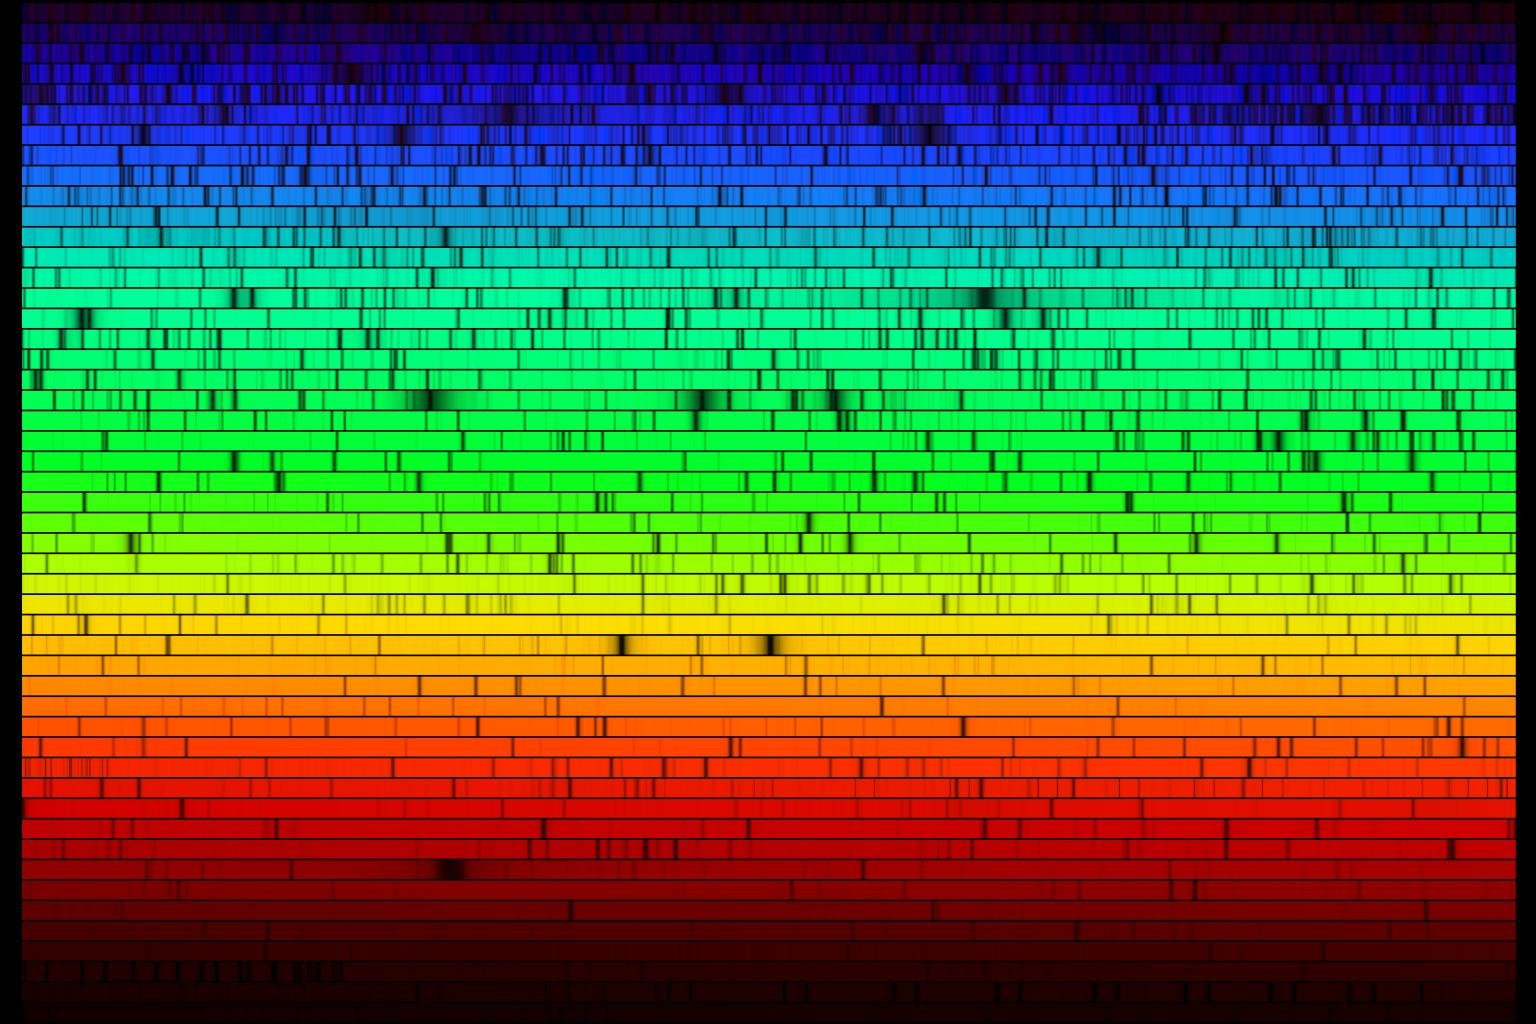
\includegraphics{'Figs/sun_spectrum.jpg'}
	\includegrpahics{'Figs/ fraunhofer-lines.gif'}
	\label{fig:fraunhofer}
	\caption{http://media.radiosai.org/journals/Vol_05/01JAN07/04-musings.htm}
\end{figure}


These lines are dark because they are absorption lines.
They are a result of the quantum mechanical effects of the electron energy shells around atoms and molecules.
In the case of the Sun, continuous white light spectrum is radiated from the photosphere, this light then interacts with the elements higher up in the atmosphere.
Upon incident with the atom or molecule, the exact wavelength of light which corresponds to the energy required to excite an electron from one energy level to another, is absorbed by the atom/molecule.
The direct result of this is that the wavelength absorbed in the energy transaction, is absent from the white light spectrum being emitted from the photosphere, and hence, appears as a dark line when observed from beyond the solar atmosphere. 

The field progressed and we began to fully understand the elements and electron transitions responsible for these abortion lines.
One of the most famous examples of these is the Balmer series, named for he man himself
This series is a set of 4 emission lines in the visible part of the Hydrogen spectrum, however, is specifically with respect to emission or absorption lines to and from energy level n = 2 as can be seen in \ref{fig:balmer}.

\begin{figure}
	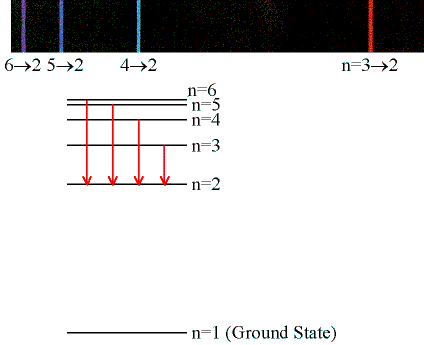
\includegraphics{'Figs/Balmer_series.gif'}
	\caption{http://www.daviddarling.info/encyclopedia/B/Balmer_series.html}
	\label{fig:balmer}
\end{figure}

Named after Johann Balmer, the transition from $n=3$ to $n=2$ is termed Hydrogen alpha (H$\alpha$), $n=4$ to $n=2$, Hyrdogen beta and so on for $n=5$ and $n=6$, gamma and delta respectively. 
However, while the concept of a simple 1-1 emission is clear, this does not always bear out in reality.
There can be environmental effects, such as temperature or magnetic field effecting the states of the energy level, which, can cause alteration of the wavelength of light emitted from the relaxation of the electron.
For instance, Hydrogen alpha is extremely useful for solar observation due to the high abundance of the atom in the atmosphere.
However, due to external factors influencing the energy levels, when we observe Hydrogen alpha, the deviation from the theoretical transition is sufficient to broaden the line to include both the upper photosphere and lower chromosphere.
Of course, Hydrogen does not just have transitions to the $n=2$, there are series associated with; $n=1$, Lyman, $n=3$, Paschen, Brackett details transitions to $n=4$ and Pfunf, $n=5$.

Clearly this methodology can be applied to all atoms and molecules that are in the solar atmosphere, allowing us to create a larger picture of the structure of the atmosphere.
We can do this by abundance and position, \emph{i.e.} there appears to be large amounts of a given transition line emission in this region and forming a structure by inspection.
As has already been said, we can associate certain transitions with various levels.
H$\alpha$ has already been discussed, moving up the atmosphere, He II $30.4$ \cite{Bazin2010} which is a Balmer-$\alpha$ transition, so $n=3$ to $n=2$, and has the same issue as H$\alpha$, in that it is extremely broad.
Calcium II and Silicon IV are both transition region, are utilised on-board the most recent space borne solar telescope, IRIS \citep{PereiraIRIS2014}. 
They are closely associated with the thin transition region, however, we do observe separate features not exclusively in the transition region.

Above the transition region Iron is bounteous, and so we have many emissions lines with which to examine the corona.
Fe VIII ($13.1$ nm), Fe IX ($17.1$ nm), Fe XII ($19.3$ nm), Fe XIV ($21.1$ nm), Fe XVI ($33.5$ nm) and Fe XVIII (9.4 nm) are all utilised on the spacecraft Solar Dynamic Observatory (SDO) with the instrument Atmospheric Imaging Assembly \cite{Schmelz2013}.
These multiple transition line from one atom are a result of the changing temperature, as it increases, the energy shells of the atoms alter, and so the various lines here apply to different temperatures.



% magnetic field recording
The energy shells of the atoms can also be effected by the environmental magnetic field, and as such we can find more out about the state of the plasma via spectroscopy as well.
The one of the effects which allows us to do this, is known as the Zeeman effect, in which, the magnetic field causes the energy levels to split based upon the spin of an electron, up or down.
The results in a splitting of what would be a single peak, into two, with the separation of the peak dependent of the size of the magnetic field present. 


\begin{figure}
	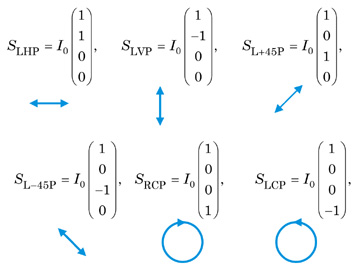
\includegraphics{Figs/stokes_params.jpg'}
	\label{stokes}
	\caption{https://spie.org/publications/fg05_p12-14_stokes_polarization_parameters. A Field guide to Polarisation.}
\end{figure}

A more suitable method by which we analyse the solar magnetic field is Stokes Polarisation Parameters.
In this method we test to what degree passing through a magnetic field has effected the electromagnetic radiation as it passes through.
In the method, the total intensity of an optical beam is defined to be a sum of three forms of polarisation, these 4 are refereed to as the polarisation parameters, I, Q, U and V.
I is raw intensity of the electromagnetic radiation, Q is the linear polarisation horizontally and vertically, U is also linearly polarized however is rotated $\pm45^\circ$ from Q and lastly V, which is polarised circularly, both left and right handed.
Using a combination of the 4 intensities it is possible to construct a vectorgram of the magnetic field and are utilised by the SDO instrument Helioseismic and Magnetic Imager (HMI) to examine features on disk.
These magnetograms are ineffective at the limb, which is a limitation of the method.
This is because a feature at the limb has no background light source to use as an origin to test the result of any polarisation. 

The vector magnetograms are used widely when studying active regions, due to the very high magnetic field strength.
They can track magnetic flux cancellation which regularly leads to the formation of other features, such as solar flares and CME's, due to the release of magnetic energy into the corona \cite{Welsch2006}.

We also observe the small magnetic bright points, which we have mentioned are observed in the photosphere and chromosphere \cite{SanchesAlmeida2010}.
They are an inherent part of what is known as the magnetic network which was visible in original measurements of the solar magnetic field over the boundaries of supergranular cells.
The magnetic field emerges from the supergranule boundaries as open magnetic field lines, extending up, into the chromosphere and above \citep{Hasan2005}.
Of course, the structure there for takes roughly the same form as the photospheric observations in G-Band,  however, with bright structures highlighting the supergranular lanes \ref{fig:mag_network}.
As a result, we have open magnetic field lines emerging with a canopy of closed magnetic field between the two boundaries.
A structure such as this can be an catalyst for physical processes such as reconnection.

It is within these regions that the magnetic bright points reside.
They appear as points of extreme intensities against the cool dark plasma of the interganular lanes, due to their intense $0.1$ T magnetic field strengths.
They are demonstrated to drift and move as the granules evolve \citep{Chitta2012} which has lead the community to suggest that these point could diffuse large amounts of heat into the solar atmosphere.

\begin{figure}
	\includegraphics{'Figs/magnetic_network_Ca_II.jpg'}
	\caption{http://science.nasa.gov/science-news/science-at-nasa/2008/02oct_oblatesun/}
	\label{fig:mag_network}
\end{figure}


\subsubsection{Coronagraphs}

Beyond $5 R_\circ$, the solar wind has become collisionless leading to minimal emissions as a result of the vastly decreased density.
Given this, we now change our approach to measure structures much further out in the corona and solar wind.
Currently, the only coronagraph still in operation is on-board the Solar Heliophysics Observatory (SoHO), the Large Angle and Spectrometric Coronagraph (LASCO). 
It is a white light detector which makes use of the effect known as Thompson Scattering which allows us to observe the particles which aren't directly emitting light off limb.
The effect entails a photon colliding with a particle, and colliding with a free charged particle in a classical sense, as opposed to a quantum interaction.
As a result of this interaction, the original photon remains unchanged in terms of energy and frequency, by this method, light from the Sun is scattered off the particles in the corona and it is this light that the coronograph detects.
In order to ensure that the detector is not washed out by the light from the Sun, ans occulting disc is essential to an operational coronagraph.


\subsection{Technology}

In the current solar observation climate, we have a wealth of information, coming from many different sources.
Understanding the functionality of these instruments in terms of the raw method is essential to rigorous science and accurate readings.

\subsubsection{Charge Coupled Devices (CCD's)}

CCD's are essential to current observational techniques and are utilised by almost every single solar mission.
They are an evolution of early photoelectric devices, which utilised the photoelectric effect, by which, a photon is incident upon a surface and an electron.
Cumulative photons exiting more electrons eventually produce a current sufficiently large to be detected.
The were known as photomultiplier devices, the drawback of which, was the restriction to a single detection per focal plane (pixel).
The primary issue with these dectectors is that they are extemely sensitive to background radiation, some on which is a result of the thermal emission from the detector.
Due to envirnomental effects cause inherent temperature of the detector to be non uniform as such the level of background can differ significantly too.
Of course, all of these effects can be corrected for, however, this will always increase the error value on the final result.

CCD's have since taken over the role which photomultipliers occupied.
Instead, CCD's are comprised of individual detectors all of high quantum efficiency arranged in a large grid, each element of which, is a single pixel.
An individual pixel keeps an electronic record of the photons striking it (summing them to an intensity).
Each pixel behaves as a potential well, trapping electrons produced as a result of the photoelectric events with the incoming photons.
The voltage resulting from the build up of electrons, is then recorded by the 

The particular advantage to a CCD is the linear response to the incoming photons \emph{i.e.} a one to one response to the incoming photons, giving extremely accurate results.
With respect to background noise and errors, the CCD is much easier to take regular dark current measurements (taking a reading with zero light coming in) and pixel to pixel variation is accounted for using flat fielding (exposing the grid to uniform field).
The gird of pixels approach also allows for much are flexibility in analysing data and correcting for the effects of events such as cosmic rays.
This is possible due to the ability to read these recordings into a computer.

\subsubsection{Ground Based telescopes}

Solar physics spent its early development being applied in ground bases solar telescopes, as has already been discussed, particularly in centres such as Royal Greenwich Observatory and Meudon Observatory in Paris.
In the modern era, the most powerful instruments, delivering high cadence and spatial resolution, are based on the ground.
Due to the challenges of observing on the ground, the location on these facilities is carefully chosen, regularly at high altitude, minimising disturbance of the signal by the atmosphere, and away from busy, polluting cities for the same reason.
The main advantages of ground based telescopes over space bourne, is that the instruments can be heavier and literally more extensive given that they do not need to be transported into space.

On La Palma in the canary islands, at $2360$ m altitude, the Swedish Solar Telescope is situated.
It utilises a $1.0$ m mirror in a refracting, vacuum solar telescope.
The vacuum is necessary due to the quantity of light the mirror reflects, causing heating which would disrupt the signal being transmitted down to a receiver.
The 'receiver' is what have become known as the optical bench, here the light beam is sent to one of several possible processing suites which are easily accessible to structure observations as needed.

SST has two such pipelines, one for the red end of the electromagnetic spectrum and another examining the blue end.
CRisp Imaging SpectroPolarimeter (CRISP), focuses on the red end of the visible spectrum, where as, the soon to be updated instrument, Chromis analyses the blue end.
The beam is split upon its arrival at the optical bench and sent to either of these instruments, however, before the beam reaches CRISP, there is a layer of correction known as adaptive optics.

Adaptive optics, corrects for atmospheric scintillation, aberration and stabilises image motion.
These cumulative effects results in an optical path difference of the light incident with the lens/mirror of the telescope.
Given this information, it is crucial to know the atmospheric physics overlying and surrounding the telescope.
It is for this reason, observatories such as the Big Bear Solar Observatory \citep{Cao2010} in Los Angeles, and the proposed new Chinese Giant Solar Telescopes \citep{Liu2014} are built on and by lakes, the reason being that the temperature will be lower, thus reducing heat haze, and therefore, atmospheric effects.
The primary atmospheric parameters influencing the set up of the adaptive optics are the Fried parameter (which measures the quality of optical transmission), the Greenwood frequency (the bandwidth required for optimal correction) and the atmospheric turbulence profile (which allows a calculation of the refractive index of the atmosphere) as shown in \cite{Rimmele2011}.

As a result of the above points, the images from the SST are extremely customisable.
They are usually returned as data cubes, with the dimensions of which are time, wavelength, x and y.
The resolution of these features are therefore changable dependant on the requirements of the observation.
Cadence can be as low as $2.5$ s, the spectral increment, $0.2$, and spatial resolution of $0.12$ arcsec.
A part of what makes this form of observation viable is the ability to directly download the received signal, which is a limitation of space borne instrumentation.
Given the possibilities of ground based observations, the method is popular, with the aforementioned Big Bear Observatory joined by a plethora of other facilities, Richard B. Dunne solar telescope (DST) in New Mexico, Mauna Loa Solar Observatory on Hawii, which will shortly be joined by the Daniel K. Inouye Solar telescope (DKIST).
DKIST promises to be the most powerful telescope ever created with a $4$ m mirror, enabling resolution of $10$ km per pixel and overcoming the quantity of photons issues at the limb for spectropolarimetry.



\subsubsection{Space Based telescopes}

Space bourne telescopes have a significant advantage over their ground based counterparts due to the nearly constant un-interrupted, view of the Sun without the atmospheric effects disturbing the signal.
As a result, the volume of space based instrumentation as grown exponentially since the early Skylab missions taking solar images from a low Earth orbit.

The first solar mission to move on from imagers on space stations was the Solar Heliospheric Observatory (SoHO).
Placed at the gravitationally stable lagrange point, L1, between the Sun and Earth, it affords constant viewing of the Sun.
It was one of the first missions to comprehensively over the entire solar environment, the instruments of which are described in \cite{StCyr}.
The science covers dopplergrams of the photosphere, EUV imaging of the chromosphere and out to LASCO, monitoring the solar wind.

Following SoHO, the Advanced Composition Explorer (ACE) \citep{Garrard1997} was placed near the L1 point as well.
It was launched in $1997$ with a much more specified goal of anaylsing the contents of the solar wind, extremely pertinent as the constituents and energy inherent in the solar wind can have extensive effects at Earth.
As a result of this, the scientific missions of ACE is heavily leant towards instrumentation which physically measures the energy and identity of a given particle.

The Solar Wind Ion Mass Spectrometer (SWICS) and Solar Wind Ion Composition Spectrometer (SWICS) are used to measure these properties.
SWICS was initially built for the ULYSSES \cite{Ulysses1992} mission which orbited the Sun in a novel slingshot orbit around jupiter, normal to the plane of orbit.

SWICS utilises a mechanical collimator to collect and direct the particles to an electrostatic deflecton array.
Whereupon, the incoming ions are deflected in accordance with the Lorentz force, $F_L = q(v x B)$.
Clearly therefore, particles incoming with higher velocities, or greater charge, will generate a larger Lorentz force, and therefore demonstrate a greater deflection when detected.
The detection is managed by a solid state detector, a semi conductor, which is applied in a similar way to CCD's.
When the particle interacts with the semiconductor, a 'charge carrier' is released.
This charge carrier is an electron currently residing in the valence band of the semi conductor, which, as a result of the particle interaction, is exited into the conduction band.
This leaves a 'hole' in the valence band, paired with the exited electron. 
The pair then migrates to opposite electrodes at either end of the semiconductor as a result of a background electric field, whereupon, they instigate a pulse which can be measured.
The amount of energy required to produce a given electron-hole pairs is known and so the particles can be inferred.

The results this instrument produced one of the most iconic set of readings in the modern era of Solar Physics.
As Ulysses completed its orbit, the radial velocity profile of the solar wind is found to vary over solar latitude.
At lower latitutes, the solar wind was found to be of the order $200$-$400$ kms$^{-1}$, before getting to higher latitudes and a distinct transition to much higher velocities.
At the time of this first orbit, the Sun was at a solar minimum, consequently, there were clear and distinct coronal holes and quiet Sun, matching with the fast and slow wind respectively.

\begin{figure}
	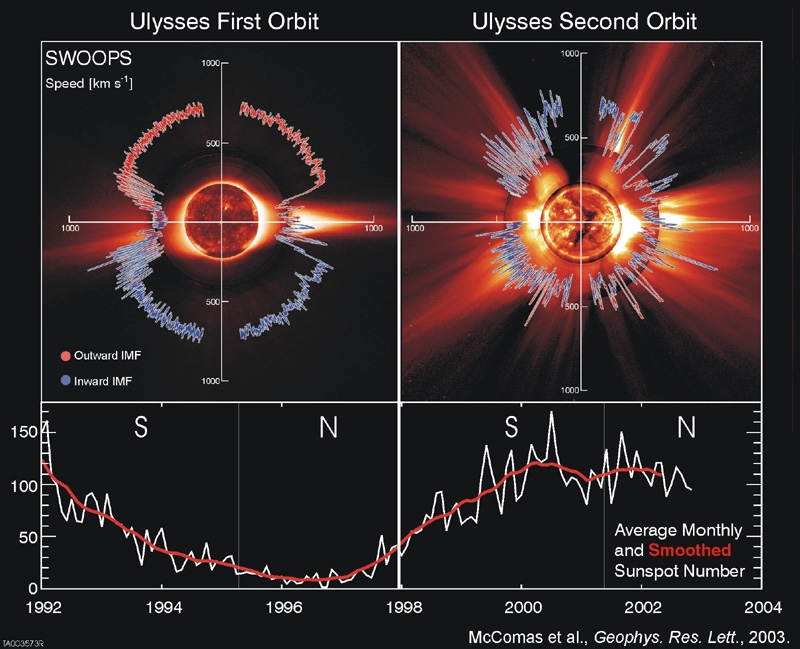
\includegraphics{Figs/ulysses_solar_wind.jpg}
	\caption{\cite{McComas2003}}
	\label{fig:ulysses_sw}
\end{figure}

The confirmation of this association between wind mode and magnetic environment came in the next orbit of Ulysses.
In this orbit, the Sun was at maximum, therefore, was almost entirely constituted of quiet Sun magnetic environments.
During this orbit, the solar wind was found to be uniformly chaotic.
Velocities are found to climb as high as those found in a fast solar wind mode, however it is not the uniformly distributed fast mode emitted from the coronal holes, as evident in the solar minima readings.

Given that we now know that the solar wind and corona have significant reach and influence, a new mission was designed and initiated, the Transition Region and Coronal Explorer (TRACE) \cite{Gaeng1998}.
As the name suggests, this instrument was designed with the specific intention on investigating the higher reaches of the solar atmosphere.
Specifically, the aim of the mission was to investigate the three dimensional structure of the low plasma beta atmosphere.
TRACE is a uniquely designed telescope, following the popular Cassegrain design, in which, the primary mirror is divided up into 4 quadrants with separate coatings in order to filter the incoming light.
This method allows simple and efficient image co-aligning.
Given that TRACE was to observe the high atmosphere, Extreme Ultra Violet lines (with the rest of the EM spectrum filtered at entrance to the detector) were selected for the imaging instruments, Fe IX $17.1$ nm, Fe XII $19.5$ nm and Fe XV $28.4$ nm.




The Japanese Aerospace Exploration Agency have organised several solar missions, Solar-A, renamed Yohkoh, \cite{Tsuneta1992} upon its successful launch and commencement of observations, pre-dates SoHO.
It covered soft and hard X-Ray ranges and spectrometers covering, specifically, the coronal Iron lines and a wide band spectrometer. 
Yohkoh was particularly successful with respect to the detection of high energy events producing large amounts of energy and X-ray emission, such as coronal jets and solar flares.
Building on the success of Yohkoh, a new mission was planned, sequentially named Solar-B and later to be renamed Hinode, sunrise in english, upon its successful launch and is presented in \cite{Kosugi2007}.
 
Hinodes launch in 2007 signified a significant move forward in space based solar observations, building from what was successful in Yohkoh.
The mission introduced small wavelength increment spectroscopy to space based missions.
The EUV Imaging Spectrometer (EIS) is designed to examine the chromospheric atmosphere using two specific imaging techniques.
It is extremely flexible with 4 slit or slot positions, $1"$ pixel slit, $2"$ pixel slit, $40"$ pixel slot and $266"$ and two different modes spectroscopy.

The spectroscopy mode 
 


Possibly the most adventurous mission to probe the solar environment is the STEREO mission (Solar TErrestrial RElations Observatory, quoted this way round due to the clear bacronym) presented in \cite{Kaiser2008}.
As is suggested by the name of this mission, the primary focus was to form a more comprehensive picture of the solar atmosphere, by positioning two satellites in such an orientation to build a three dimensional picture.
Consequently, two identical satellites were launched into \emph{solar} orbits, ahead and behind the orbit.
There is an inherent differential in the angular velocity of the spacecraft, in order to move the spacecraft ever further around the orbit at approximately $45^\circ$ per year.
The primary objective of this stage of the mission was to obtain the optimal angle to produce three dimensional images of the Sun using a tomographic technique.

Given that STEREO was designed to give varying angles of the solar-earth  enviroment, the instruments on the mission are tailored to this need.
SECCHI is a suite of 5 imagers, utilising white light chronographs, an extreme ultra violet imager and two wide angle Heliospheic Imagers (HI) designed to track CME's to $1$ AU.
IMPACT detects solar wind electrons and in situ solar wind magnetic field strength and vector, while PLASTIC measures composition of heavy ions, alpha particles and protons. 
Given the instumentation, STEREO is used extensively by space weather forecasters at NOAA, which, will increasingly become and essential part of our lives.

Building on all of the above missions, the Solar Dynamic Observatory (SDO) mission begun in 2010 \cite{Kaiser2008}.
The instruments are developments of concepts used on previous missions but expanding them to allow constant viewing of the entire solar disk.
Consequently all instruments on SDO view the full solar disk, at all times, maintaining the same temporal cadence. 
Therefore, the SDO mission produces significantly more raw data than any previous, from an purely engineering standpoint, the instruments were carefully selected to facilitate the downloading of the data.
As such, SDO has three scientific aims; the Helioseismic and magnetic Imager (HmI) examining the solar variability and finer scale structure of the solar magnetic field; Extreme Ultraviolet Variability Experiment (EVE) measured the total solar irradiance in the Extreme Ultra Violet section of the spectrum and the Atmospheric Imaging Assembly (AIA) investigating the upper chromosphere and corona.

AIA's imaging suite provides full disk images in $4096 \times 4096$ resolution and most importantly at $12$ second cadence.
However, its distinguishing feature is the array of wavelengths analysing the atmosphere \cite{AIAspec} associated with various temperatures equivalent to the appropriate electron transitions.
The instrument ranges through $170$, $30.4$, $160$, $17.1$, $19.3$, $21.1$, $33.5$, $9.4$ and $13.1$ nm providing a temperature range of $5000$ K to $1.6 \times 10^7$ K.




\section{Plasma behaviour}

Stars are incredibly unique features, their behaviour is entirely unlike any planetary body, and has already been discussed, their inherent magnetic field makes their structure extremely complex.All of these affects can be traced back to the fact that the Sun consists of gas kept at high temperature and pressure, which causes it to form the $4^{th}$ state of matter, plasma.
Plasma is defined as a gas in which the molecules reached an energy level that cause them to eject their outermost electrons and become Ions, causing the gas to be a neutral mixture of charged Ions and free electrons (produced from ionising the molecules).
It can be formed in several situations, such as a discharge of current from the atmosphere to the ground, manifesting as lightening as the propagating current ionises the air.

The motion and behaviour of a plasma can be defined on small scales but 3 factors; The plasma approximation, bulk interaction and the plasma frequency.
The plasma approximation states that the particles must be close enough together such that any given particle must influence all particles within the Debye screening length.
The length is dependant on the permittivity of free space, the Boltzmann constant, electron charge, temperatures of the Ions and electrons, density of electrons and density of an atomic species.

\begin{equation}
	\lambda_D = \sqrt{(\epsilon_0\kappa_BT_e)/(n_eq_e^2)}
\end{equation}

Bulk interaction refers to the statement that the Debye screening length is small compared to the overall scale of the plasma, this implies that the motion of the interior guides the characteristic behaviour, rather than motion at the edges.
Lastly the plasma frequency refers to the oscillation of the elections within the plasma, which is valid if this frequency is higher than the collions between electrons and neutrals.
In this case, the electrostatic interactions dominate over the standard, gas-like behaviour we would otherwise see.
Of course, the case where all the molecules or atoms are ionised is the ideal case, however, in nature this is not always true.
The degree of the ionisation is defined in terms of the ratio of ions to electrons, $\alpha = n_i/{n_i + n_n}$ where $i$ is the number density of ions and $n$ for neutrals.

As is evident from the Debye screening length, the temperture of the plasma, can have a dominating effect on the characteristics of the plasma.
The temperature is a measure of the thermal kinetic energy of the plasma, clearly higher kinetic energy therefore equates to a higher temperature of the plasma.
However, electrons will reach a thermal equillibrium significantly faster than the ions and neutrals, in which situation the plasma will have two, or even three, populations.
In the case where the plasmas electrons and ions in thermal equilibrium with the neutrals the plasma is termed, shockingly enough, thermal.
In nonthermal plasmas, the electrons, whose temperatures raise quicker, will be at a higher temperature than the heavier ions and neutrals.
The degree of ionisation of the plasma that results a thermal equilibrium us given by the following;

\begin{equation}
	x^2/{x - 1} = (2\pim_e)^{3/2}/h^3 (\kappa_BT)^{5/2}/p_{gas} exp(-{\chi/\kappa_BT}), \cite{Saha1920}
\end{equation}

Where $p_{gas}$ is the gas pressure, $m_e$ is the mass of the electron amd $\chi$ is the ionisation energy.
This form of the Saha ionisation equation will hold for Hydrogen, however does not take into account multiple ionisation processes, as would be the case for a more complex atom or molecules.
The result of this is that degree of ionisation in a gas will increase with increases in temperature.
It therefore follows that not all plasmas are fully ionised, at lower temperatures, the heavier elements won't gain enough energy to ionise, sometimes despite the fact that the electrons are orders of magnitude higher in temperature.

Given that plasma behaves differently, we therefore need a set of laws to define how the plasma behaves on scales such as those applicable on the Sun and in the atmosphere.


\subsection{MHD}

Magnetohydrodynamics are the set of laws by which we describe the motion of plasma on scales.
They were derived by \cite{Alfven1942}, an achievement for which, Alfv{\'e}n was awarded the nobel prize.	
The rules set up are a combination of the gas pressure equations and Maxwell's laws of electrodynamics, so let us now examine this relationship.

When considering a plasma, it is important to remember that while the total charge of the plasma will be quasi-neutral, the ions and electrons which constitute the mixture still carry charge.
Consequently, motions in the plasma will cause the charges to have a change in velocity.
In accordance with Farady's law, a moving charge will cause a magnetic field to be induced and Ohms' law will also become a factor with charges moving through a magnetic field.
As such, this can be an extremely complex problem, let us begin our discussion with Maxwell's equations;

\begin{equation}
	\divv \times \mb{E} = -\pd{\mb{B}}{t} & & \textnormal{Faradys}
	
	\divv \times \mu_0\mb{j} + \frac{1}{c^2}\pd{\mb{E}}{t} & & \textnormal{Amp{\`e}re}
	
	\divv{\mb{E}} = \frac{\tau}{\epsilon_0} & & \textnormal{Gauss'}
	
	\divv{\mb{B} = 0} & & \textnormal{Gauss' law of magnetism}
\end{equation}

where $\mb{E}$ is the electric field stength, $\mb{B}$ the magnetic field, $t$ is time, $c^2 = (\epsilon_0\mu_0)^{-1}$,$\epsilon_0$ is the vacuum permittivity, $\mu_0$ is the permeability of free space, $\mb{j}$ is the current density and $\tau$ is the charge density.
Faraday's law describes how a changing magnetic field would induced an electric field, hence it is also known as the Induction equation.
Amp{\`e}re's law describes the manner in which the magnetic field integrated around a closed loop, related to the electric current passing through said loop.
Gauss' law for magnetism is also known as the Solenoidal condition and states that no magnetic monopoles exist and the eponymous law describes the resulting electric field caused by an electric charge.

The second `half' of the magnetohydrodynamic equations are the laws for gas dynamics, expressed in terms of the partial derivatives;

\begin{equation}
	\pd{\rho}{t} + \del \cdot (\rho\mb{v}) = 0 & & \textnormal{Equation of mass conservation}
	
	\pd{p}{t} + \mb{v\cdot}\divv{p} + \gamma p\divv{\cdot}\mb{v} = 0 & & \textnormal{Conservation of entropy}
\end{equation}

in Eulerian time-dervative reference frame, evaluated for a fixed position within the fluid.
In the case of these two sets of equations, there is currently no link other than the velocity vector, $\mb{v}(\mb{r},t)$ which can be introduced through the equation of motion for a fluid element.
The equation for the motion of the fluid element is derived from the rate of change of momentum equations 

\begin{equation}
	$\frac{d}{dt}\int_{V}^{}dV\rho\mb{v} = \int_{V}^{}dV\rho\td{\mb{v}}{t} = rate of change of momentum$
\end{equation}

In this case the rate if change of momentum will equal the net force on the fluid element, in accordance with newtons second law, therefore;

\begin{equation}
	\rho \td{\mb{v}}{f} = \rho\mb{g} + \divv{\cdot}[X]
\end{equation}

where X is the total of all forces exerted on the fluid element. 
Therefore the equation which will incorporate all of these terms and calculate the acceletation on a fluid element is:

\begin{equation}
	\rho \td{\mb{v}}{t} = \mb{F} \equiv -\divv{p} + \rho\mb{g} + \mb{j} \times \mb{B + \tau\mb{E}} 
\end{equation}

As we are currently assuming that we have a totally ionised fluid, therefore the electric field is defined as

\begin{equation}
	\mb{E}' \equiv \mb{E} + \mb{v} \times \mb{B} = 0
\end{equation}

and therefore, $\mb{E}'$ in a co-moving frame will vanish.
The last assumption we need to make, is that the velocity of the plasma is not relativistic $v \ll c$.

This allows us to make some assertions as to the scale of the terms in Amp{\`e}re's equation, the length scales of $l_0$ and $t_0$ are shown such that $v = l_0/t_0$.
This means we can negelect the displacement current from Amp{\`e}re's and define the current $\mb{j}$ purely in terms of \mb{B}:

\begin{equation}
	\mb{j} = \frac{1}{\mu_0}\del \times \mb{B}
\end{equation}

As a result of which, we can neglect the effects of space charge on the plasma.
Additionally, the non-relativistic assumption means that we can also make a simplification to the acceleration of a fluid element equation as the electrostatic acceleration is small, as well, Gauss' can be dropped through lack of need.
As such the electric field can expressed merely in terms of the velcoity and magneticfield vectors:

\begin{equation}
	\mb{E} = -\mb{v} \times \mb{B}
\end{equation}

But applying the above assumptions, and substituteing in for $\mb{E}$ and $\mb{j}$, we obtain the basic equations of ideal magnetohydrodynamics.

\begin{equation}
	\pd{\rho}{t} + \del\cdot(\rho\mb{v}) = 0
	
	\rho(\pd{\mb{v}}{t} + \mb{v}\cdot\divv{\mb{v}}) + \divv{p} - \rho\mb{g} - \frac{1}{\mu_0}(\del \times \mb{B}) \times \mb{B} = 0
	
	\pd{p}{t} + \mb{v}\cdot\divv{p} + \gammap\del\cdot\mb{v} = 0
	
	\pd{\mb{B}}{t} - \del \times (\mb{v} \times \mb{B}) = 0
	
	\del\cdot\mb{B}
\end{equation}








\subsection{Reconnection}

\section{Jet and Macrospicules}

The appearance of thin, explosive features with a relatively short lifespan has always been a part of solar physics.
Spicules were first observed in 1877 by a vatican observer, Angelo Secchi.
This was aided by their sheer ubiquity, they were distinctly visible at the solar limb nearly all the time.
However the larger scale, more infrequent jets are more difficult to observe, particularly with early solar observations.

\subsection{The ejecta zoo}

The wide variety of jets and jet like feature 
Jets and jet like features are observed throughout the solar atmosphere, and as such a review of the topic is in order.
As has already been discussed, spicules are the smallest jets formed in the solar atmosphere, 
most easily observed at the limb, they are long thin structure appearing brightly at the solar limb \citep{Beckers1972}.
Spicules are found in the chromosphere, regularly observed in the H$\alpha$, He II $30.4$ nm, Ca II and Si IV.
Work by \cite{DePontieu} divided spicules into two populations, Type-1 and Type-2, with Type-1 being long lived and Type-2 having distinctly shorter lifetimes, but however are significantly more explosive and grow to much higher lengths .
Type-1 spicules have an uprising speed of approximately $20$ kms$^{-1}$ and extend to $1$ Mm in height, whereas the Type-2 spicules have been shown to extend approximately $5$ Mm into the atmosphere and last for an average of $10$ minutes.
The most comprehensive difference between the two is in the overall evolution of the feature.
Type 1 spicules are observed to have a parabolic evolution \emph{i.e.} their tip traced out a ballistic arc when plotted against time.
Conversely, Type II spicules are observed to dissipate or vanish as they evolve, and are primarily observed in the quiet Sun and coronal holes, Type I develop in active regions, as such, Type II are far more numerous when recorded in a study such as \cite{Pereira2012}.

\begin{figure}
	\includegaphics{'Figs/spicules_at_limb.jpg'}
	\caption{http://www.nasa.gov/sites/default/files/images/751917main_highres4_full.jpg Spicules as observed by Hinode}
\end{figure}

Spicules are visible on the disk as well, however, on disk we see dark thin structures against the bright lower chromosphere, these were initially named mottles and fibris, however have since been inherently linked with spicules, see \cite{DePointeu2007MF}.

Since these initial propositions, however, there has been doubt cast as to whether this is the case or not. 
Cite Zhang 2010 found no statistical separation of populations within spicules and recent publications but the original authors have shown that Type-2 spicules disappear from Ca II and reappear in the hotter Si IV and Mg II lines \citep{Pereira2014}.
This would imply that spicules are heating as they accelerate through the atmosphere, whether this is because the underlying formation mechanism is different or there is sufficient energy in the initialisation of the spicule to cause heating as they propagate through the atmosphere, has yet to be made clear.

The formation of spicules is still a matter of much debate given our currently limited ability to examine small scales in current observations. 
However, when observations are unable to provide explict results, numerical and analytic approaches are utilised to fill in the gaps.
\cite{DePointeu2004} outline a mechanism for the formation of spicules which originates in the photosphere.
P-mode oscillations cannot pass through the photosphere due to the minimum temperature, however, evanescence allows the waves to propogate into the higher atmosphere, where higher temperatures allow propagation to restart.
Also essential to this model is the inclination of the native magnetic field.
The authors report that the inclined field, vastly increases the likelihood of waves tunneling through the atmosphere. 
In the lower density solar atmosphere causes the photospheric velocity generated by the p-modes to leak into the atmosphere and steepen into shocks, which leave and oscillating wake in the chromosphere, the spicule.

However this is only one of many competing theories, \cite{Takeuchi2001}, demonstrate a magnetic reconnection model driving formation of spicules, whereas \cite{Martinez2011} formed a $3$ dimensional model utilising the Lorentz force to push plasma across the solar surface until it meets vertical magnetic field which forces the plasma upwards.
\cite{Hollweg1982} demonstrate a quasi-impulsive source in the photosphere is capable of generating a chain of rebound shocks in the chromosphere, causing the formation of a spicule.

A particularly pertinent model is proposed by \cite{Moore2011spic_recon}, in which magnetic reconnection is instigated by granule sized 'magnetic bubbles'.
This is applicable, as spicules are generally observed to form on the intergranular lanes.
The authors propose that Type 2 spicules are an analogue for X-ray jets (more on which later).
In this scenario, magnetic bipoles emerge from the photosphere which then interacts with the ambient field of the lower chromosphere, forming a raft of reconnection external to the bipole.
During this reconnection, the interior of the bipole remains inert while the outer most sections of the structure, 'sling shot snapping' of the magnetic reconnected field lines produce; an upward jet (Type II spicule), Alfven waves propagating up the ambient magnetic field lines and a fast MHD wave upwards across the magntic field.

The advantages of this scenario for connection is that the environment which generates these spicules, is eminently reproducible throughout the solar surface.
The scenario here is particularly convenient as it also answers questions with respect to heating of the solar atmosphere.
As a result of the 'canopy region' that forms over the granules reconnecting with the more open magnetic fields higher in the atmosphere, causing shocks and waves to propagate upwards.
The dissipation of the energy within these disturbances, has been proposed on numerous occasions to be the central source of heating of the corona.  

What becomes evident, after all of these models are formed, none of them generate both Type I and type II spicules, therefore it is likely that they are indeed two separate features.


Throughout the solar atmosphere, we observe much larger jet-like features than spicules.
They have been observed extensively, and not solely in the chromosphere.
The first observations of more large scale jet were undertaken using the Soft X-Ray telescope on board Yohkoh \citep{Tsuneta1991}.
\cite{Shimojo1996} undertook the first statistical study of jets, finding a nice round $100$ examples to study.
With any study looking for specific features, the authors utilised the following selection criteria; 1) That the plasma is collimated and that the movement of the feature was in the direction of the collimation, 2) The aspect ratio of length to width is greater than $3$ and 3) The time between the pre-jet image and the image in which the jet first appears is less than an hour.
These are an excellent example of selection criteria which aide in forming the search, however, are vague enough not to introduce bias into the sample.

The authors find that the jets are primarily formed with a microflare/sub flares at the base/footpoints (the terms are used interchangeably in literature).
They find their lengths to be of the order $10$ - $400$ Mm and widths are of the order $5$-$500$ Mm.
Velocities along the direction of collimation we observed to range between $10$ and $1000$ kms$^{-1}$, averaging at approximately $200$ kms$^{-1}$ lifetimes extending to $10$ hours.
In terms of physical evolution of their shapes, the authors find that $76\%$ of the jets demonstrated converging shapes, \emph{i.e.} the width of the jet would be constant over its evolution or decreasing with distance from the footpoint. The constant form were found to come from a wide variety of energy sources, whereas the converging form, explicitly formed from energetic points. 
This work has formed the basis of much of the study of jet phenomena, however, this is merely an exploratory study around which future studies have explored.

% possibly more required here

What has become known as the standard model for the formation of solar jets is demonstrated  by \cite{Shibata1992}.
Within this paper, the authors use the Soft X-Ray telescope on Yohkoh to examine $20$ jets, and present their spatial properties, very similar to those of \cite{Shimojo1996}, however, the authors go on to describe a possible formation schematic.
The model is based upon the flux emergence from the lower solar atmosphere, and is backed up by data in the Solar Geophysical Data.
The authors demonstrate that the observations reveal a void at the jet base, similar in appearance to voids observed in reconnection driven events such as flares and CME's.
The authors proposed that the jets are based in the chromosphere based on an inspection of the emission measure, consequently it is likely that the mass is from the chromosphere.
The authors propose that the undulating and meandering shape of the jet lends itself to a helically twisting magnetic structure, suggesting that the jet itself emanates from a relaxation of the magentic field along a global flux tube \cite{Shibata1986}.
Such a reconnection event between twisted and untwisted magnetic field, would be capable of producing a jet of this size, lifetime, and more importantly, velocity.

This model for the standard jet requires that there be open magnetic field lines, and a smaller scale, twisted, emgering flux loop to rise from the lower atmosphere in order to initiate a reconnection event.
As a result of the reconnection event, material in the emerging loop is than transfered into the open magnetic field lines, 'sling shotting' around the loop it as formerly a part of and up the open field lines, thus revealing the collimated beam of plasma.
The mechanism highlighted in this particular model produces exclusively narrow jets, a couple of mega meters in width.
It also results in the dissipation of large amounts of energy which manifests as brightenings in may observations.
From the source of the reconnection, energised plasma then dissipates down the loops highlighting the entire feature.
The visual effect of the long collimated beam/plasma spire and the newly brightened loop of plasma, reveals an 'inverted - Y' shape or Eiffel tower like structure, similar to the 'cusp' shape observed in significantly larger features high in the corona round streamers and flares \cite{Vourlidas2006}.
These terms have gained common usage in literature and will be used hereafter. 

An excellent example of this type of formation is demonstrated in \cite{Nishizuka2011}.
Within this work, the authors demonstrate what is refereed to as an Anemone jet, so called as the dome like bipole magnetic bubble, may be viewed as a feature similar to the sea creature.
The model they build as a result of this is in three dimensions, consequently, the small scale loops of the standard model could be projected into $3$D as an anemone-like shape.
The authors observed the jet in Ca II, it formed along an inclined line approximately $45^\circ$ away from normal, in the inverted-y format.
With the jet forming in Ca II, we can conclude that this particular jet is formed in the upper chromosphere, with this particular jet the authors observe the formation loop itself.
The jet feature is found to extend $14$ Mm into the atmosphere and its width, $6$ Mm, with maximum velocity observed at $100$ kms$^{-1}$, however, $10$ minutes into the evolution of the jet, contrary to what you might expect.

The standard jet model accurately describes a prominent section of the jet population, however, those which it does not cover is highlighted in \cite{Moore2010}.
The specific example that the standard jet model does not cover is the case where the width of the jet is more than that predicted by the standard model.
\cite{Moore2010} utilise Hinode/XRT to look for X-ray jets occuring in the polar coronal holes, and where possible the authors observed the same features in EUVI as well.

The initial magnetic field topology is largely similar to that of the standard jet, a small scale loop with open magnetic field extending upwards.
The difference in these models is that the emerging bipole arch in the case of the standard jet, remains untwisted and without shear.
In the case of blowout jets, this arch/loop is sufficiently twisted and sheared that it can drive an explosive eruption.
In terms of the physical evolution, there is no difference between the two until the emerging flux element triggers a reconnection burst at the boundary between said emerging flux and the open magnetic field lines.

The authors then go on to suggest two resolutions to the reconnection event; that the boundary becomes unstable on its own, and consequently reconnection begins on its own.
This results in beakout reconnection, expelling the loops outer magnetic field, which lifts the restriction on sheared flux lower in the system; consequently allowing the core of the emerging flux to erupt upwards. 
This forms a chain event, with emerging core events causing more reconnection and consequent releases and so on, similar to \cite{Antiochos1998}.
The second permutation, is that the sheared core, begins to erupt before any reconnection takes place at the boundary.
In this scenario, an instability in the emerging bipole causes the previously stable core to begin emerging.
As a result, magnetic pressure at the boundary current sheet between the loop and open magnetic loop, eventually triggering breakout reconnection.

This work clearly has impact on the current relationships between the various jets of scales larger than spicules (which clearly are their own feature.)
The authors propose that the blowout jets correspond to the macrospicule features in the chromosphere, more on which later.
As for implications with respect to the division of standard and blowout jets, observations of the formation mechanism would clarify the feature.
Standard jets would have large originating loop spanning approximately $20$ Mm or not visible at temperatures lower than  $10^6$ K.
Whereas, blowout jets need to produce strong signals in H$\alpha$ and He $30.4$, due to the cooler plasma thrown upwards from the unstable magnetic bipole emerging.

One of the most comprehensive sets of jet observations is undertaken by \cite{Majarska2011}, in which, the authors observe a jet in an equatorial coronal hole.
Utilising, SUMER on SoHO, EIS and XRT on Hinode and the EUVI instruments on the STEREO A and B.
The authors find that the jet can be heated my microflares at the moment of reconnection, rising the temperature up to $12$ MK.
This was obtained using a DEM technique integrating the emission from a range of spectral lines to estimate the temperature, and the density was approximated at $4 \times 10^9$ cm$^{-3}$ using a similar technique.
http://www.aanda.org/articles/aa/pdf/2011/02/aa15269-10.pdf


% This section may need to go else where
What becomes clear is that these large scale jets can only be trigger by explosive reconnection events, therefore understanding this mechanism is essential to out understanding of solar jets.
\cite{Archontis2005} demonstrate the mechanism governing the rules of this interaction.









Jets
Other than standard jet model Shibata
Anenome Jets - Nishivuka
A general discussion Archontis http://iopscience.iop.org/article/10.1086/497533/meta
Stat study of network jets http://arxiv.org/abs/1604.06295


Chromospheric Jets




\subsection{Macrospicules}


The subject of this thesis is a clarification of the classification of macrospicules. 
They are features not dissimilar to jets, however they have been distinguished from the population of jets in the current literature, which will now be discussed below.

Macrospicules were first reported by \cite{Bohlin1975}, utilising the SkyLab mission.
This was undertaken using $30.4$ nm instrument making observations of the polar coronal holes.
The initial images were taken as raw light through particular filters over the lens, the images were also over exposed in order accentuate the appearance of the solar limb.
The authors found that the newly named macrospicule was visible in He II $30.4$, however was not apparent in Ne VII $46.5$ nm or Mg IX $36.8$ nm, observing the transition region and corona respectively.
The authors then classify macrospuicules accornding to 3 observables; that the macrospicules are confined to the coronal holes; that the macrospicules increasingly inclined away from normal proportionally to their distance from the solar pole and the authors link this to the supposedly weak, inclined magnetic field again; and lastly that they are only visible in $30.4$ nm.
 
% possibly wack in a frame of the 'frames'

The authors specifically differentiate between the H$\alpha$ spicules previously observed, stating that these new features have no counterpart in that line, citing work by Engvold and Beckers 1975 unable to find a correlation between the two lines by direct observation or numerical correlation.
Having said this, they make the caveat that there is a possibility that the formations of the two features, could be largely similar.

With the limitations of the observations at the time, there was much debate as to whether this was actually the case. 
Following up on the work by Bohlin, \cite{LaBonte79} utilised the Big Bear Solar Observatory to examine the 'limb surges' in H$\alpha$ and Deuterium 3 (D$_3$).
The authors found that the macrospicules in H$\alpha$ had considerable complexity in their structure, with 'knots, twists and loops' within the confines of the feature.
But in D$_3$, the authors only observe the brightest parts of the macrospicule, usually at the base of the structure apparent in H$\alpha$.
Differently in this case, the authors also observe features on the disk and define three categories, the macrospicules appearing similar to filament eruptions, surge-like macrospicules and a flare brightening type.
Lastly the paper finds that the rate of occurrence of macrospicules to be of the order $~1400$ per solar day. 
This discussion as to the possible links between the two features goes on to this day, more on which later.

The next seminal work on macrospicules was published in \cite{Dere89}, again using an early space station, SpaceLab 2, as the platform for space based observations.
In this case a Gregorian telescope was used to take a series of broadband UV observing at the solar limb.
As a result of this set up the images are a convolution of the intensities from the solar continuum, therefore, differentiating between structures is not possible.
This means that only macrospicules spactial extent be observed, and specifically those which appeared above the limb, with no study of their onset.
Consequently, this study is statistical in its focus with the aim being to ascertain the basic spacial properties of the population.

The authors then go on to compare the values obtained in this study to the two previously mentioned. The papers are generally in agreement, specifically Dere and LaBonte, citing lengths ranging between $5$ - $33$ arcsec and similar widths, although Dere et al. find $3$ - $9$ arcsec and LaBonte $0.7$ - $6$.
The question of velocities is also raised, values quoted as $20$ - $50$ kms${^{-1}}$ from Dere et al. and $\leq60$ kms${^{-1}}$ from LaBonte.
Although these values should possibly be taken with a pinch of salt as the temporal resolution for Dere and Labonte was $20$ or $60$ s and $1$ min respectively, which will greatly influence the measurement of the velocity.
However, Bohlin et al. find more extreme values for all of the studies.
Some of the lengths they find, extend as far as $60$ arc sec, greater widths, $5$ - $15$ arcsec and velocities reaching $150$ kms${^{-1}}$, although, again the temporal resolution is poor, $\geq~180$ s.
Although this early work had its limitations, the groundwork was laid here in order to be more precise when more sophisticated missions would be undertaken in the mid $90$'s with a focus on detail and less so on statistical properties.

With the launch of SoHO in 1996, the community now had continuous viewing of the solar disk, meaning that consistent observations of macrospicules is now possible.
On of the first studies utilising the new instruments was undertaken by \cite{Pike1997} using the Coronal Diagnostic Spectrometer (CDS).
In this case, the instrument scanned from north to south pole, using a mosaic of rastered images, using the He I $58.433$ nm, O V $62.973$ nm and Mg IX $36.806$ lines, corresponding to temperatures of $20,000$, $250,000$ and $1,000,000$ K.
In this case the macrospicule is apparent at the limb, demonstrating two brightpoints visible in the footpoints either side of the structure, and a fainter column of plasma extending off the limb.
The authors find that the macrospicule is visible in the He I and O V lines, however not in the higher temperature magnesium line, showing that macrospicules can be found at, and above, transition region temperatures.
The authors find the macrospicule to be $31$ Mm in height and $13.3$ Mm in width, agreeing with previous values.

The bright roots evident in the O V lines begin to form the 'inverted-Y' shape, typical of the standard jet formation mechanism outlined by Shibata.
As a result of this the authors go on to discuss the nature of the feature and whether it is a macrospicule or X-ray jet.
The authors conclude that this feature is still classified as a macrospicule, due to the observations in He I and the feature adhering to the properties highlighted in \cite{Bohlin1976}.

Building on the work done by Pike, \cite{Parenti2002} undertook an extremely detailed case study of a macrospicule observed in CDS.
In this case the observations are still reliant on the macrospicule protruding above the limb, using the full suite of spectra available to the authors.
When discussing these papers, we must consider the rastering method of CDS.
The images are comprised of vertical columns of pixels that are exposed for $30 $ s, has a cooldown phase before moving onto the next vertical slit. 
This takes approximately $240$ s, which is inappropriate for a feature which on average doesn't have a large lifespan.
Therefore, the pixels in the x direction, from one column to the next, are separated by a time of $272$ s.
This means that we cannot consider the spatial structure in the x direction as continuous.
As a result of this the authors use the columns of the image array as temporal cadence of the macrospicule. 

The authors find that the macrospicule extends to $26$ Mm and reaches an maximum velocity of $81.6$ kms${^{-1}}$ and an average outflow velocity of $26$ kms${^{-1}}$.
The spectroscopic nature of CDS allows for the calculation of temperature and density.
As the full range of CDS's GIS suite is being used, the density is not strictly a single number and will be dependent on the emission in the various wavelenghts.
The density is highest in O IV, $~1.5 \times 10^10$ and varies throught the lines but generally dropping to the order of $10^8$ by the Si IX line.
The temperatures are calculated as rations between emission lines, \emph{e.g.} O V $62.97$ nm / O IV $55.45$ nm. giving values around $2.0 \times 10^5$ K, which the authors demonstrate is hotter than the surrounding atmosphere at that point, agreeing with previous works by \cite{Habbal1991}.



As instrumentation improved, the use os spectroscopy resulted in the discovery of the rotational behaviour of a macrospicule as demonstrated in \cite{Kamio2010}.
In this case, the authors are utilising STEREO-A, the hinode mission and SUMER. 
STEREO used to observe the feature in $30.4$ for straight forward imaging, hinode for dopplergrams and XRT and SUMER for spectroscopic data.

In the lead up to the particular case the study examines, there were multiple coronal jets occurring at the source of the macrospicule over a $9$ hour period.
When the macrospicule erupted, again apparent were two foot-points at the base of the feature in the $30.4$ nm STEREO images, however, in this study there is also a brightening in XRT at the same time. 
This is one of the first concrete examples of the relationship between macrospicules and X-ray jets.
The authors then go on to highlight that the two foot-points then go on to form two threads emanating upwards, into the corona, subsequently utilising the SUMER instrument to detect their motion in detail.

The properties of this particular example in He II $30.4$ are quoted at $130 \pm 30$ kms${^{-1}}$ for the radial extension of the feature and line of sight velocities of the order $-15$ and $-25$ kms${^{-1}}$.
With respect to the X-ray jet behaviour, the velocity is measured at $320 \pm 30$ kms${^{-1}}$ and utilising the LoS velocity in He VIII and Fe XII lead the authors to conclude that the structure of the macrospicule and X-ray jet. 
The authors also highlight the regression of the material back to the limb causing an enhancement in He II, a phenomena they propose is caused by either heating in the upper part of the feature or a result of the density increase caused by the down flow of plasma.

The helical motion of macrospicules is observed in multiple papers, \cite{Curdt2011} present observations of macrospicules in the transition region.
In this case the authors present two examples of 'explosive events', in one case the feature is on the disk and in the second is above the limb.
The discussion at the heart of the paper is differentiating between RRE/RBE pairs and helical motion, due to the fact that they can be misinterpreted in the data. 
In this case, the rotational velocity evident in the doppler images demonstrates symmetrical flow of the order $40$ kms${^{-1}}$ for both examples.
Using the slit modes of EIS, the authors rule out the possibility of lateral movement as a result of bidirectional RRE/RBE's, calculating that if this were the case, then the jet would be up to $7.2$ Mm in each doppler component.
This leads to the conclusion that the jet evident at the limb is moving helically, and consequently, that the feature observed on the disk is also a single jet rotating helically.

The development of spectosopic analysis in the most recent generation of solar observational technology, is highlighted in \cite{Scullion2010}, again in the context of on, and off limb macrospicules. 
























 
































\begin{pycode}[chapter1]
from __future__ import print_function

ch1 = texfigure.Manager(pytex, number=1, base_path='./Chapter1/')
\end{pycode}

\begin{pycode}[chapter1]
fig = plt.figure(dpi=100, figsize=texfigure.figsize(pytex, height_ratio=1.5))

xx = np.linspace(0, 6*np.pi, 1000)
plt.plot(xx, np.sin(xx))

fig.tight_layout()
fig.subplots_adjust(bottom=0.15)
photosphere = ch1.save_figure('sin', fig, fext='.pgf')
photosphere.caption = "Some sine wave."
\end{pycode}

\py[chapter1]|photosphere|



Hello world, checkout \cref{fig:sin}.


\begin{pycode}[chapter1]
	
multi = texfigure.MultiFigure(4,1)
width = 0.9

X = [[5,6], [7,8], [5,6], [7,8]]
Y = [[1,2], [3,4], [1,2], [3,4]]

for x,y in zip(X,Y):
	fig = plt.figure(figsize=texfigure.figsize(pytex, scale=width))
	plt.plot(x, y, 'o')
	
	Fig1 = ch1.save_figure('test', fig)
	Fig1.subfig_width=r"{}\columnwidth".format(width)
	multi.append(Fig1)
\end{pycode}

\py[chapter1]|multi[0:2]|
\py[chapter1]|multi[2:4]|
